\newif\ifglobal

%%%%%%%%%%%%%%%%%%%%%%%
%%% Compile to view %%%
%%%%%%%%%%%%%%%%%%%%%%%

%%%%%%%%%%%%%%%%%%%%%%%%%%%%%%%%%%%%%%%%%%%%%%%%%%%
%%% Readme:                                     %%%
%%% https://www.overleaf.com/read/bwdjvfjksvjy/ %%%
%%%%%%%%%%%%%%%%%%%%%%%%%%%%%%%%%%%%%%%%%%%%%%%%%%%

% >>> M?: marks a module setting number or important notice

% >>> M4: Set {./relative-path} to external files for this module <<<
\def \modulefiles {./20-SENSOR}
% To add an external file, use:
% (Replace '---' with actual filename)
% '\input{\modulefiles/tables/---.tex}' for tables
% '\includegraphics{\modulefiles/figures/---}' for figures
% '\subfile{\modulefiles/---}' for register files


% >>> M1: This module is in global project? <<<
% 'YES' - uncomment; 'NO' - comment out
\globaltrue

\ifglobal
    \documentclass[main\_\_EN.tex]{subfiles}
   
\else
    \documentclass[openany, 10pt]{book}

    % >>> M2: In ./00-shared/preamble-trm-module, also find
    %         settings for visibility of todo notes, watermark <<<
    \usepackage{preamble-trm-module}
\usepackage{ctex}
    % >>> M3: Temporary labels in English,
    %         you can add your own labels there <<<
    \myexternaldocument{./00-shared/temp-labels-en}

\fi %\ifglobal


\setcounter{secnumdepth}{4}


% >>> M5: If this module needs any updates in
% './00-shared/preamble-trm-module.sty'
% (include additional package, etc.), contact your module PM
% or create the file './00-shared/changelog.tex' make the
% necessary updates yourself and document them in this file <<<


\begin{document}


% Sets language into which pre-defined bits of text are translated
\selectlanguage{english}

% Do not delete this block
\ifglobal
% Add the following front matter if
% this module is outside of global project
\else
    \InputIfFileExists{readme}{}{}
    {\let\clearpage\relax \listoftodos}
    \tableofcontents
    %\listoftables
    %\listoffigures
\fi

%%%%%%%%%%%%%%%%%%%%%%%%%
%%% Chapter status: this is the latest document. Please update this document directly if there is any updates in future%%%
%%%%%%%%%%%%%%%%%%%%%%%%%

%%%%%%%%%%%%%%%%%%%%%%%%%
%%% TRM Module Begins %%%
%%%%%%%%%%%%%%%%%%%%%%%%%

\hypertarget{sensor}{}
\chapter{On-Chip Sensor and Analog Signal Processing}
\label{mod:sensor}

\section{Overview}

\chipname{} provides the following on-chip sensor and analog signal processing peripherals:

\begin{itemize}
    \item Two 12-bit Successive Approximation ADCs (SAR ADCs): SAR ADC1 and SAR ADC2, for measuring analog signals from six channels.
    \item One temperature sensor for measuring the internal temperature of the \chipname{} chip.
\end{itemize}

\section{SAR ADCs}\label{sec:sensor-sar-adc}

\subsection{Overview}

\chipname{} integrates two 12-bit SAR ADCs, which are able to measure analog signals from up to six pins. The SAR ADCs are managed by two dedicated controllers:

\begin{itemize}
    \item DIG ADC controller: drives  \hyperref[other:sensor-item-read-data-from-sar-adc1]{Digital\_Reader0} and  \hyperref[other:sensor-item-read-data-from-sar-adc1]{Digital\_Reader1} to sample channel voltages of SAR ADC1 and SAR ADC2, respectively. This DIG ADC controller supports high-performance multi-channel scanning and DMA continuous conversion.
    \item PWDET controller: monitors RF power. Note this controller is only for RF internal use.
\end{itemize}

\begin{tiplisting}
The DIG ADC controller of SAR ADC2 for \chipname{} does not work properly and it is suggested to use SAR ADC1. For more information, please refer to \href{\linkprefix\linkchiperrataEN}{\chipseries{} Series SoC Errata}.
\end{tiplisting}

\subsection{Features}
\begin{itemize}
\item Each SAR ADC has its own ADC Reader module (\hyperref[other:sensor-item-read-data-from-sar-adc1]{Digital\_Reader0} or  \hyperref[other:sensor-item-read-data-from-sar-adc1]{Digital\_Reader1}), which can be configured and operated separately. 
\item Support 12-bit sampling resolution
\item Support sampling the analog voltages from up to six pins

\item DIG ADC controller:
    \begin{itemize}
        \item Provides separate control modules for one-time sampling and multi-channel scanning. 
        \item One-time sampling and multi-channel scanning can be run independently on each ADC.
        \item Channel scanning sequence in multi-channel scanning mode is user-defined.
        \item Provides two filters with configurable filter coefficient.
        \item Supports threshold monitoring. An interrupt will be triggered when the sampled value is greater than the pre-set high threshold or less than the pre-set low threshold.
        \item Supports DMA
    \end{itemize}
\item PWDET controller: monitors RF power (for internal use only)
\end{itemize}


\subsection{Functional Description}

The major components of SAR ADCs and their interconnections are shown in Figure  \ref{fig:sensor-sar-adc-function-overview}.

\begin{figure}[H]
    \centering
    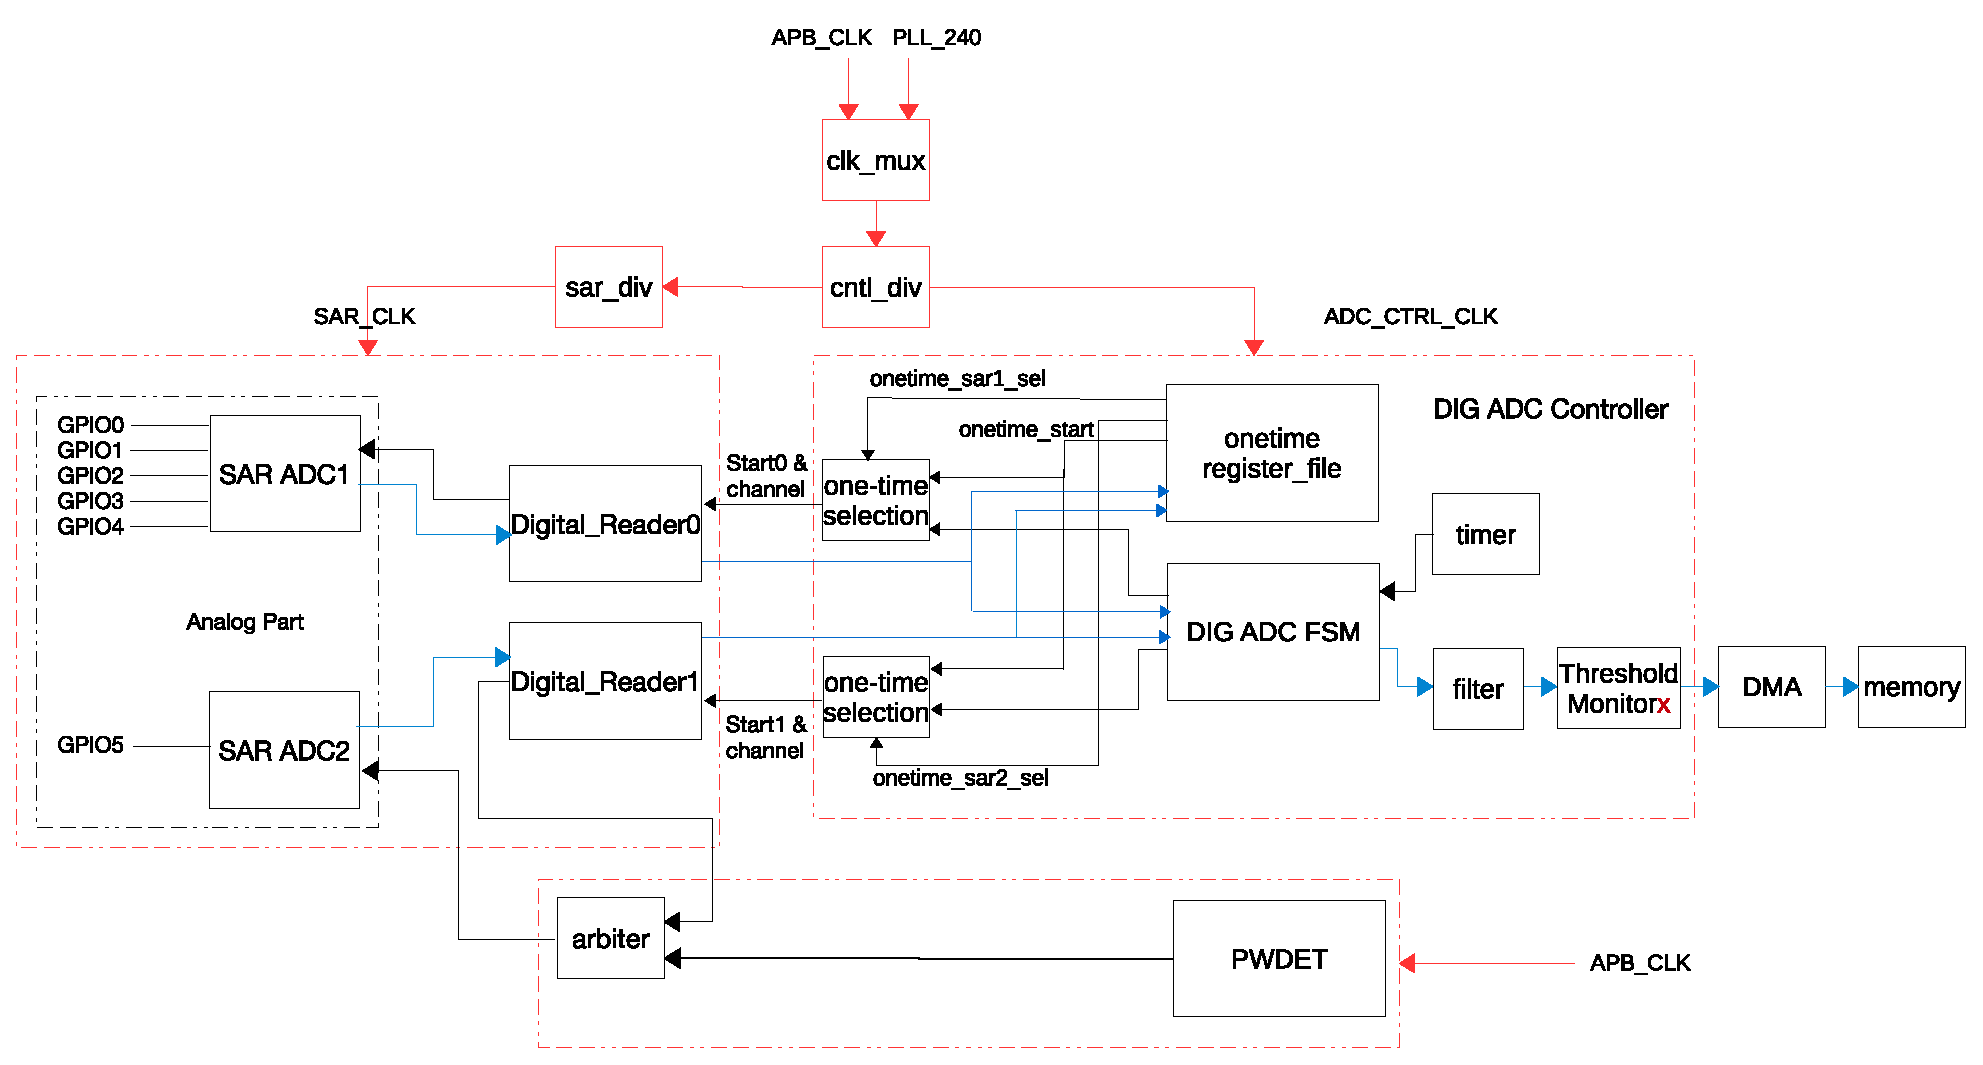
\includegraphics[width=1.1\textwidth]{./20-SENSOR/figures/on_chip_sensor_20240606}
    \textcolor{blue}{\textbf{---}}: data flow; \textcolor{red}{\textbf{---}}: clock signal; \textcolor{black}{\textbf{---}}: ADC control signal
    \caption{SAR ADCs Function Overview}
    \label{fig:sensor-sar-adc-function-overview}
\end{figure}

As shown in Figure  \ref{fig:sensor-sar-adc-function-overview}, the SAR ADC module consists of the following components:

\begin{itemize}
    \item SAR ADC1: measures voltages from up to five channels.
    \item SAR ADC2: measures the voltage from one channel. 
    \item Clock management: selects clock sources and their dividers:
        \begin{itemize}
            \item Clock sources: can be APB\_CLK or PLL\_240.
            \item Divided Clocks:
             \begin{itemize}
                 \item SAR\_CLK: operating clock for SAR ADC1, SAR ADC2, Digital\_Reader0, and Digital\_Reader1. Note that the divider (sar\_div) of SAR\_ADC must be no less than 2.
                 \item ADC\_CTRL\_CLK: operating clock for DIG ADC FSM.
             \end{itemize}
        \end{itemize}
    \item Arbiter: this arbiter determines which controller is selected as the ADC2's working controller, DIG ADC controller or PWDET controller.
    \item \label{other:sensor-item-read-data-from-sar-adc1} Digital\_Reader0 (driven by DIG ADC FSM): reads data from SAR ADC1.
    \item Digital\_Reader1 (driven by DIG ADC FSM): reads data from SAR ADC2.
    \item DIG ADC FSM: generates the signals required throughout the ADC sampling process.
    \item Threshold monitor\regindex{x}: threshold monitor 1 and threshold monitor 2. The monitor\regindex{x} will trigger a interrupt when the sampled value is greater than the pre-set high threshold or less than the pre-set low threshold.
\end{itemize}
The following sections describe the individual components in details.

\subsubsection{Input Signals}

In order to sample an analog signal, an SAR ADC must first select the analog pin to measure via an internal multiplexer. A summary of all the analog signals that may be sent to the SAR ADC module for processing by either ADC1 or ADC2 are presented in Table \ref{tab:sensor-sar-adc-input-signals}.

\begin{longtable}{ |p{2.5cm}|p{1.5cm}|p{2.5cm}| }
    \caption{SAR ADC Input Signals}
    \label{tab:sensor-sar-adc-input-signals}
    \\\hline
    \rowcolor{lightgray}
    Signal  & Channel  & ADC Selection \\ \hline
    \endfirsthead
    \hline
    \rowcolor{lightgray}  
    Signals  & Channels  & ADC Selection \\ \hline
    \endhead
    \hline
    \endfoot
    GPIO0       &  0  & \multirow{5}{*}{SAR ADC1} \\ \cline{1-2}
    GPIO1       &  1  & \\ \cline{1-2}
    GPIO2       &  2  & \\ \cline{1-2}
    GPIO3       &  3  & \\ \cline{1-2}
    GPIO4       &  4  & \\ \cline{1-3}
    GPIO5       &  0  & SAR ADC2 \\ \hline
\end{longtable}

\subsubsection{ADC Conversion and Attenuation}

When the SAR ADCs convert an analog voltage, the resolution (12-bit) of the conversion spans voltage range from 0 mV to \(V_{ref}\). \(V_{ref}\) is the SAR ADC's internal reference voltage (1100 mV by design). The output value of the conversion (data) is mapped to analog voltage \(V_{data}\) using the following formula:

    \[
    V_{data} = \frac{V_{ref}}{k}\times{\frac{data}{4095}}
    \]

\(k\) is the coefficient corresponding to the configured attenuation.

In order to convert voltages larger than \(V_{ref}\), input signals can be attenuated before being input into the SAR ADCs. The supported attenuation levels are:

\begin{itemize}
    \item 0 dB (k≈100\%)
    \item 2.5 dB (k≈75\%)
    \item 6 dB (k≈50\%)
    \item 12 dB (k≈25\%)
\end{itemize}

\subsubsection{DIG ADC Controller}

The clock of the DIG ADC controller is quite fast, thus the sample rate is high. For more information, see Section ADC Characteristics in \href{https://www.espressif.com/sites/default/files/documentation/esp32-c3_datasheet_en.pdf}{\chipname{} Series Datasheet}. 

This controller supports: 

\begin{itemize}
    \item up to 12-bit sampling resolution
    \item software-triggered one-time sampling
    \item timer-triggered multi-channel scanning
\end{itemize}

The configuration of a one-time sampling triggered by the software is as follows:
\begin{itemize}
    \item Select SAR ADC1 or SAR ADC2 to perform a one-time sampling:
    \begin{itemize}
        \item if \hyperref[fielddesc:APBSARADCSARADC1ONETIMESAMPLE]{APB\_SARADC1\_ONETIME\_SAMPLE} is set, SAR ADC1 is selected.
        \item if \hyperref[fielddesc:APBSARADCSARADC1ONETIMESAMPLE]{APB\_SARADC2\_ONETIME\_SAMPLE} is set, SAR ADC2 is selected.
    \end{itemize}
    \item Configure \hyperref[fielddesc:APBSARADCSARADCONETIMECHANNEL]{APB\_SARADC\_ONETIME\_CHANNEL} to select one channel to sample.
    \item Configure \hyperref[fielddesc:APBSARADCSARADCONETIMEATTEN]{APB\_SARADC\_ONETIME\_ATTEN} to set attenuation.
    \item Configure \hyperref[fielddesc:APBSARADCSARADCONETIMESTART]{APB\_SARADC\_ONETIME\_START} to start this one-time sampling.
    \item On completion of sampling, \hyperref[fielddesc:APBSARADCAPBSARADC2DONEINTRAW]{APB\_SARADC\_ADC\regindex{x}\_DONE\_INT\_RAW} interrupt is generated. Software can use this interrupt to initiate reading of the sample values from \hyperref[fielddesc:APBSARADCAPBSARADC1DATA]{APB\_SARADC\_ADC\regindex{x}\_DATA}. \regindex{x} can be 1 or 2. 1: SAR ADC1; 2: SAR ADC2.
\end{itemize}

If the timer-triggered multi-channel scanning is selected, follow the configuration below. Note that in this mode, the scan sequence is performed according to the configuration entered into pattern table. 
\begin{itemize} 
        \item Configure  \hyperref[fielddesc:APBSARADCSARADCTIMERTARGET]{APB\_SARADC\_TIMER\_TARGET} to set the trigger target for DIG ADC timer. When the timer counting reaches two times of the pre-configured cycle number, a sampling operation is triggered. For the working clock of the timer, see Section \ref{other:sensor-para-dig-adc-clock}.
        \item Configure  \hyperref[fielddesc:APBSARADCSARADCTIMEREN]{APB\_SARADC\_TIMER\_EN} to enable the timer.
        \item When the timer times out, it drives DIG ADC FSM to start sampling according to the pattern table;
        \item Sampled data is automatically stored in memory via DMA. An interrupt is triggered once the scan is completed.
\end{itemize}

\begin{tiplisting}
Any SAR ADC can not be configured to perform both one-time sampling and multi-channel scanning at the same time. Therefore, if a pattern table is configured to use any SAR ADC for multi-channel scanning, then this SAR ADC can not be configured to perform one-time sampling.
\end{tiplisting}

\subsubsection{DIG ADC Clock}\label{other:sensor-para-dig-adc-clock}
Two clocks can be used as the working clock of DIG ADC controller, depending on the configuration of \hyperref[fielddesc:APBSARADCCLKSEL]{APB\_SARADC\_CLK\_SEL}:
\begin{itemize}
    \item 1: Select the clock (ADC\_CTRL\_CLK) divided from PLL\_240.
    \item 0: Select APB\_CLK.
\end{itemize}

If ADC\_CTRL\_CLK is selected, users can configure the divider by \hyperref[fielddesc:APBSARADCCLKMDIVNUM]{APB\_SARADC\_CLKM\_DIV\_NUM}. Note that due to speed limits of SAR ADCs, the operating clock of Digital\_Reader0, SAR ADC1, Digital\_Reader1, and SAR ADC2 is SAR\_CLK, the frequency of which affects the sampling precision. The lower the frequency, the higher the precision. SAR\_CLK is divided from ADC\_CTRL\_CLK. The divider coefficient is configured by \hyperref[fielddesc:APBSARADCSARADCSARCLKDIV]{APB\_SARADC\_SAR\_CLK\_DIV}.

The ADC needs 25 SAR\_CLK clock cycles per sample, so the maximum sampling rate is limited by the SAR\_CLK frequency.

\subsubsection{DMA Support}

DIG ADC controller supports direct memory access via peripheral DMA, which is triggered by DIG ADC timer. Users can switch the DMA data path to DIG ADC by configuring \hyperref[fielddesc:APBSARADCAPBADCTRANS]{APB\_SARADC\_APB\_ADC\_TRANS} via software. For specific DMA configuration, please refer to Chapter \ref{mod:dma} \textit{\nameref{mod:dma}}.

\subsubsection{DIG ADC FSM}
\textbf{Overview}

Figure \ref{fig:sensor-diagram-dig-adc-fsm} shows the diagram of DIG ADC FSM.

\begin{figure}[H]
    \centering
    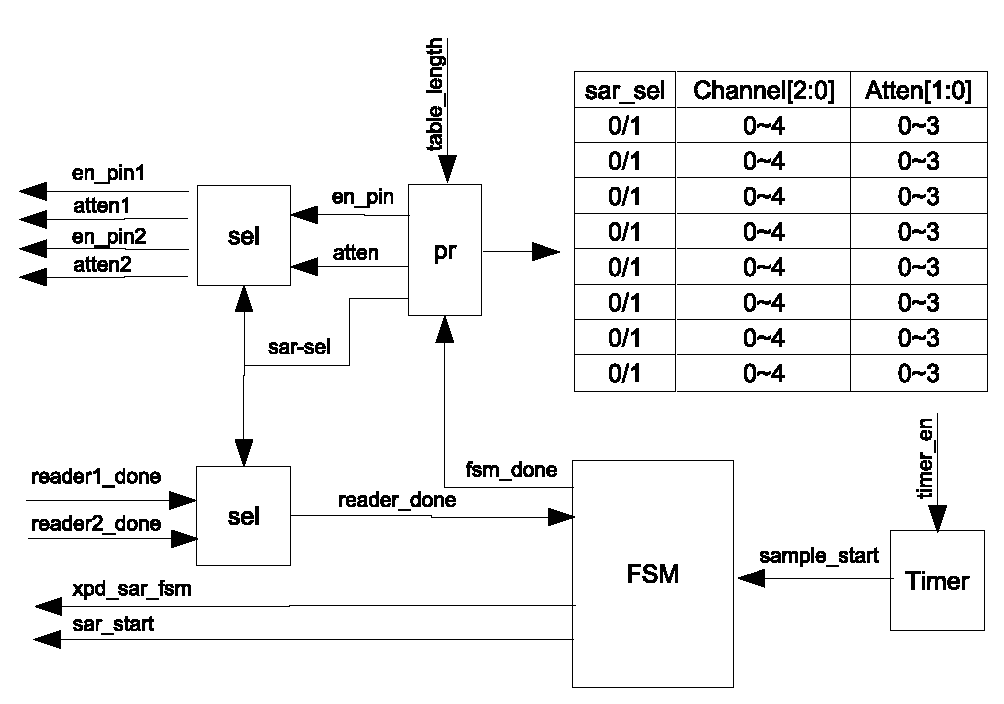
\includegraphics[width=0.7\textwidth]{./20-SENSOR/figures/20-sensor-saradc_dma_20210901}
    \caption{Diagram of DIG ADC FSM}
    \label{fig:sensor-diagram-dig-adc-fsm}
\end{figure}

Wherein:
\begin{itemize}
    \item Timer: a dedicated timer for DIG ADC controller, to generate a sample\_start signal.
    \item pr: the pointer to pattern table entries. FSM sends out corresponding signals based on the configuration of the pattern table entry that the pointer points to.
\end{itemize}

The execution process is as follows:
\begin{itemize}
\item Configure  \hyperref[fielddesc:APBSARADCSARADCTIMEREN]{APB\_SARADC\_TIMER\_EN} to enable the DIG ADC timer. The timeout event of this timer triggers an sample\_start signal. This signal drives the FSM module to start sampling.
\item When the FSM module receives the sample\_start signal, it starts the following operations:
\begin{itemize}
    \item Power up SAR ADC.
    \item Select SAR ADC1 or SAR ADC2 as the working ADC, configure the ADC channel and attenuation, based on the pattern table entry that the current pr points to.
    \item According to the configuration information, output the corresponding en\_pad and atten signals to the analog side.
    \item Initiate the sar\_start signal and start sampling.
\end{itemize}

    \item When the FSM receives the reader\_done signal from ADC Reader (Digital\_Reader0 or Digital\_Reader1), it will
    \begin{itemize}
        \item stop sampling,
        \item transfer the data to the filter, and then threshold monitor transfers the data to memory via DMA,
        \item update the pattern table pointer pr and wait for the next sampling. Note that if the pointer pr is smaller than \hyperref[fielddesc:APBSARADCSARADCSARPATTLEN]{APB\_SARADC\_SAR\_PATT\_LEN} (table\_length), then pr = pr + 1, otherwise, pr is cleared.
    \end{itemize}
\end{itemize}    
    



\textbf{Pattern Table}

There is one pattern table in the controller, consisting of the \hyperref[regdesc:APBSARADCSARPATTTAB1REG]{APB\_SARADC\_SAR\_PATT\_TAB1\_REG} and \hyperref[regdesc:APBSARADCSARPATTTAB1REG]{APB\_SARADC\_SAR\_PATT\_TAB2\_REG} registers, see Figure \ref{fig:sensor-apb-saradc-sar-patt-tab1-reg-pattern-tab-entry0-entry3} and Figure \ref{fig:sensor-apb-saradc-sar-patt-tab2-reg-pattern-tab-entry4-entry7}:

\regfield{(reserved)}{8}{24}{00000000}%
\regfield{cmd3}{6}{18}{{0x0000}}%
\regfield{cmd2}{6}{12}{{0x0000}}%
\regfield{cmd1}{6}{6}{{0x0000}}%
\regfield{cmd0}{6}{0}{{0x0000}}%
\begin{regdesc}\begin{reglist}
\item [cmd \regindex{x}] represents pattern table entries. \regindex{x} here is the index, 0 \verb+~+ 3.
\end{reglist}\end{regdesc}
\vspace{-2em}
\begin{figure}[H]
    \centering
    \caption{APB\_SARADC\_SAR\_PATT\_TAB1\_REG and Pattern Table Entry 0 - Entry 3}
    \label{fig:sensor-apb-saradc-sar-patt-tab1-reg-pattern-tab-entry0-entry3}
\end{figure}

\regfield{(reserved)}{8}{24}{00000000}%
\regfield{cmd7}{6}{18}{{0x0000}}%
\regfield{cmd6}{6}{12}{{0x0000}}%
\regfield{cmd5}{6}{6}{{0x0000}}%
\regfield{cmd4}{6}{0}{{0x0000}}%
\begin{regdesc}\begin{reglist}
\item [cmd \regindex{x}] represents pattern table entries. \regindex{x} here is the index, 4 \verb+~+ 7.
\end{reglist}\end{regdesc}
\vspace{-2em}
\begin{figure}[H]
    \centering
    \caption{APB\_SARADC\_SAR\_PATT\_TAB2\_REG and Pattern Table Entry 4 - Entry 7}
    \label{fig:sensor-apb-saradc-sar-patt-tab2-reg-pattern-tab-entry4-entry7}
\end{figure}

Each register consists of four 6-bit pattern table entries. Each entry is composed of three fields that contain working ADC, ADC channel and attenuation information, as shown in Table  \ref{fig:sensor-pattern-table-entry}.


\begin{figure}[H]
\centering
\regfield{sar\_sel}{1}{5}{{x}}%
\regfield{ch\_sel}{3}{2}{{xx}}%
\regfield{atten}{2}{0}{xx}%
\end{figure}
\vspace{-2em}
\begin{figure}[H]
    \centering
    \caption{Pattern Table Entry}
    \label{fig:sensor-pattern-table-entry}
\end{figure}
\vspace{-2em}
\begin{regdesc}\begin{reglist}
\item [atten] Attenuation. 0: 0 dB; 1: 2.5 dB; 2: 6 dB; 3: 12 dB.
\item [ch\_sel] ADC channel, see Table \ref{tab:sensor-sar-adc-input-signals}.
\item [sar\_sel] Working ADC. 0: SAR ARC1; 1: SAR ADC2.
\end{reglist}\end{regdesc}





\textbf{Configuration of multi-channel scanning}

In this example, two channels are selected for multi-channel scanning:
\begin{itemize}
    \item Channel 2 of SAR ADC1, with the attenuation of 12 dB
    \item Channel 0 of SAR ADC2, with the attenuation of 2.5 dB
\end{itemize}

The detailed configuration is as follows:

\begin{itemize}
    \item Configure the first pattern table entry (cmd0):

\centering
\regfield{sar\_sel}{1}{5}{{0}}%
\regfield{ch\_sel}{3}{2}{{2}}%
\regfield{atten}{2}{0}{3}%
\reglabel{}\regnewline%
\begin{regdesc}\begin{reglist}
\begin{figure}[H]
    \centering
    \caption{cmd0 Configuration}
\end{figure}
\vspace{-2em}
\item [atten] write the value of 3 to this field, to set the attenuation to 12 dB.
\item [ch\_sel] write the value of 2 to this field, to select channel 2 (see Table \ref{tab:sensor-sar-adc-input-signals}).
\item [sar\_sel] write the value of 0 to this bit, to select SAR ADC1 as the working ADC.
\end{reglist}\end{regdesc}
\end{itemize}

\begin{itemize}
    \item Configure the second pattern table entry (cmd1):

\centering
\regfield{sar\_sel}{1}{5}{{1}}%
\regfield{ch\_sel}{3}{2}{{0}}%
\regfield{atten}{2}{0}{1}%
\reglabel{}\regnewline%
\begin{regdesc}\begin{reglist}
\begin{figure}[H]
    \centering
    \caption{cmd1 configuration}
\end{figure}
\vspace{-2em}
\item [atten] write the value of 1 to this field, to set the attenuation to 2.5 dB.
\item [ch\_sel] write the value of 0 to this field, to select channel 0 (see Table \ref{tab:sensor-sar-adc-input-signals}).
\item [sar\_sel] write the value of 1 to this bit, to select SAR ADC2 as the working ADC.
\end{reglist}\end{regdesc}
\end{itemize}

\begin{itemize}
    \item Configure \hyperref[fielddesc:APBSARADCSARADCSARPATTLEN]{APB\_SARADC\_SAR\_PATT\_LEN} to 1, i.e., set pattern table length to (this value + 1 = 2). Then pattern table entries cmd0 and cmd1 will be used. 
    \item Enable the timer, then DIG ADC controller starts scanning the two channels in cycles, as configured in the pattern table entries.
\end{itemize}

\textbf{DMA Data Format}

The ADC eventually passes 32-bit data to the DMA, see the figure below.

\begin{figure}[H]
\centering

\regfield{reserved}{15}{17}{{xx}}%
\regfield{sar\_sel}{1}{16}{{x}}%
\regfield{ch\_sel}{3}{13}{{xxx}}%
\regfield{reserved}{1}{12}{{x}}%
\regfield{data}{12}{0}{xx}%
\end{figure}
\vspace{-2em}
\begin{figure}[H]
    \centering
    \caption{DMA Data Format}
    \label{fig:sensor-dma-data-format}
\end{figure}
\vspace{-2em}
\begin{regdesc}\begin{reglist}
\item [data] SAR ADC read value, 12-bit
\item [ch\_sel] Channel, 3-bit
\item [sar\_sel] SAR ADC selection, 1-bit
\end{reglist}\end{regdesc}



\subsubsection{ADC Filters}
The DIG ADC controller provides two filters for automatic filtering of sampled ADC data. Both filters can be configured to any channel of either SAR ADC and then filter the sampled data for the target channel. The filter's formula is shown below:

\[data_{cur} = \frac{(k-1)data_{prev}}{k}+\frac{data_{in}}{k}+0.5\]

\begin{itemize}
    \item \(data_{cur}\): the filtered data value.
    \item \(data_{in}\): the sampled data value from the ADC.
    \item \(data_{prev}\): the last filtered data value.
    \item \(k\): the filter coefficient.
\end{itemize}

The filters are configured as follows:
\begin{itemize}
\item Configure \hyperref[fielddesc:APBSARADCAPBSARADCFILTERCHANNEL1]{APB\_SARADC\_FILTER\_CHANNEL\regindex{x}} to select the ADC channel for filter \regindex{x};
\item Configure \hyperref[fielddesc:APBSARADCAPBSARADCFILTERCHANNEL1]{APB\_SARADC\_FILTER\_FACTOR\regindex{x}} to set the coefficient for filter \regindex{x};
\end{itemize}

Note that \regindex{x} is used here as the placeholder of filter index. 0: filter 0; 1: filter 1.

\subsubsection{Threshold Monitoring}
DIG ADC controller contains two threshold monitors that can be configured to monitor on any channel of SAR ADC1 and SAR ADC2. A high threshold interrupt is triggered when the ADC sample value is larger than the pre-configured high threshold, and a low threshold interrupt is triggered if the sample value is lower than the pre-configured low threshold.

The configuration of threshold monitoring is as follows:
\begin{itemize}
    \item Set \hyperref[fielddesc:APBSARADCAPBSARADCTHRESALLEN]{APB\_SARADC\_THRES\regindex{x}\_EN} to enable threshold monitor \regindex{x}.
    \item Configure \hyperref[fielddesc:APBSARADCAPBSARADCTHRES1LOW]{APB\_SARADC\_THRES\regindex{x}\_LOW} to set a low threshold;
    \item Configure \hyperref[fielddesc:APBSARADCAPBSARADCTHRES1LOW]{APB\_SARADC\_THRES\regindex{x}\_HIGH} to set a high threshold;
    \item Configure \hyperref[fielddesc:APBSARADCAPBSARADCTHRES1LOW]{APB\_SARADC\_THRES\regindex{x}\_CHANNEL} to select the SAR ADC and the channel to monitor.
\end{itemize}

Note that \regindex{x} is used here as the placeholder of monitor index. 0: monitor 0; 1: monitor 1.

\subsubsection{SAR ADC2 Arbiter}

SAR ADC2 can be controlled by two controllers, namely, DIG ADC controller and PWDET controller. To avoid any possible conflicts and to improve the efficiency of SAR ADC2, \chipname{} provides an arbiter for SAR ADC2. The arbiter supports fair arbitration and fixed priority arbitration.

\begin{itemize}
    \item Fair arbitration mode (cyclic priority arbitration) can be enabled by clearing  \hyperref[fielddesc:APBSARADCADCARBFIXPRIORITY]{APB\_SARADC\_ADC\_ARB\_FIX\_\\PRIORITY}.
    \item In fixed priority arbitration, users can set \hyperref[fielddesc:APBSARADCADCARBAPBPRIORITY]{APB\_SARADC\_ADC\_ARB\_APB\_PRIORITY} (for DIG ADC controller) and  \hyperref[fielddesc:APBSARADCADCARBWIFIPRIORITY]{APB\_SARADC\_ADC\_ARB\_WIFI\_PRIORITY} (for PWDET controller), to configure the priorities for these controllers.
 A larger value indicates a higher priority.
\end{itemize}


The arbiter ensures that a higher priority controller can always start a conversion (sample) when required, regardless of whether a lower priority controller already has a conversion in progress. If a higher priority controller starts a conversion whilst the ADC already has a conversion in progress from a lower priority controller, the conversion in progress will be interrupted (stopped). The higher priority controller will then start its conversion. A lower priority controller will not be able to start a conversion whilst the ADC has a conversion in progress from a higher priority controller.  

Therefore, certain data flags are embedded into the output data value to indicate whether the conversion is valid or not.

\begin{itemize}
    \item The data flag for DIG ADC controller is the \{sar\_sel, ch\_sel\} bits in DMA data, see Figure \ref{fig:sensor-dma-data-format}.
    \begin{itemize}
        \item 4'b1111: Conversion is interrupted.
        \item 4'b1110: Conversion is not started.
        \item Corresponding channel No.: The data is valid.
    \end{itemize}
    \item The data flag for PWDET controller is the two higher bits of the sampling result.
    
    \begin{itemize}
        \item 2'b10: Conversion is interrupted.
        \item 2'b01: Conversion is not started.
        \item 2'b00: The data is valid.
    \end{itemize}
\end{itemize}
Users can configure  \hyperref[fielddesc:APBSARADCADCARBGRANTFORCE]{APB\_SARADC\_ADC\_ARB\_GRANT\_FORCE} to mask the arbiter, and set  \hyperref[fielddesc:APBSARADCADCARBWIFIFORCE]{APB\_SARADC\_ADC\_ARB\_WIFI\_FORCE} or \hyperref[fielddesc:APBSARADCADCARBAPBFORCE]{APB\_SARADC\_ADC\_ARB\_APB\_FORCE} to authorize corresponding controllers.

\section{Temperature Sensor}\label{sec:sensor-temp-sensor}
\subsection{Overview}
\chipname{} provides a temperature sensor to monitor temperature changes inside the chip in real time.

\subsection{Features}
The temperature sensor has the following features:
\begin{itemize}
    \item Supports software triggering and, once triggered, the data can be read continuously
    \item Configurable temperature offset based on the environment, to improve the accuracy
    \item Adjustable measurement range
\end{itemize}


\subsection{Functional Description}

The temperature sensor can be started by software as follows:
    \begin{itemize}
        \item Set \hyperref[fielddesc:APBSARADCTSENSPU]{APB\_SARADC\_TSENS\_PU} to start XPD\_SAR,
        and then to enable temperature sensor;
        \item Set \hyperref[fielddesc:SYSTEMTSENSCLKEN]{SYSTEM\_TSENS\_CLK\_EN} to enable temperature sensor clock;
        \item Wait for \hyperref[fielddesc:APBSARADCTSENSXPDWAIT]{APB\_SARADC\_TSENS\_XPD\_WAIT} clock cycles till the reset of temperature sensor is released, the sensor starts measuring the temperature;
        \item Wait for a while and then read the data from \hyperref[fielddesc:APBSARADCTSENSOUT]{APB\_SARADC\_TSENS\_OUT}. The output value gradually approaches the actual temperature linearly as the measurement time increases.
    \end{itemize}



The actual temperature (°C) can be obtained by converting the output of temperature sensor via the following formula:
\[
        T(°C) = 0.4386 * VALUE – 27.88 * offset – 20.52
\]

VALUE in the formula is the output of the temperature sensor, and the offset is determined by the temperature offset. The temperature offset varies in different actual environment (the temperature range). For details, refer to Table \ref{tab:tsensor-dac}.

\begin{longtable}[c]{|p{4cm}|p{4cm}|}
    \caption{Temperature Offset}
    \label{tab:tsensor-dac}
    \\\hline
    \rowcolor{lightgray}
    Measurement Range (°C)  & Temperature Offset (°C) \\\hline
    50 \verb+~+ 125 & -2 \\\hline
    20 \verb+~+ 100 & -1 \\\hline
    -10 \verb+~+ 80 & 0 \\\hline
    -30 \verb+~+ 50 & 1 \\\hline
    -40 \verb+~+ 20 & 2 \\\hline
\end{longtable}

\section{Interrupts}

\begin{itemize}
   \item \label{interreupt:SARADCDONEINT1} APB\_SARADC\_ADC1\_DONE\_INT: Triggered when SAR ADC1 completes one data conversion.
   \item \label{interreupt:SARADCDONEINT2} APB\_SARADC\_ADC2\_DONE\_INT: Triggered when SAR ADC2 completes one data conversion.
   \item \label{interreupt:APBSARADCTHRESxHIGHINT} APB\_SARADC\_THRES\regindex{x}\_HIGH\_INT: Triggered when the sampling value is higher than the high threshold of monitor \regindex{x}.
    \item \label{interreupt:APBSARADCTHRESxLOWINT} APB\_SARADC\_THRES\regindex{x}\_LOW\_INT: Triggered when the sampling value is lower than the low threshold of monitor \regindex{x}.
\end{itemize}


\section{Register Summary}

The addresses in this section are relative to the ADC controller base address provided in Table \ref{tab:sysmem-base-address} in Chapter \ref{mod:sysmem} \textit{\nameref{mod:sysmem}}.

The abbreviations given in Column \textbf{Access} are explained in Section \hyperref[glossary-access-types]{\textit{Access Types for Registers}}.

\subfile{\modulefiles/apb_saradc_sw_pass_reg_summary_20210409_eng}

\section{Register}

The addresses in this section are relative to the ADC controller base address provided in Table \ref{tab:sysmem-base-address} in Chapter \ref{mod:sysmem} \textit{\nameref{mod:sysmem}}.

\subfile{\modulefiles/apb_saradc_sw_pass_reg_20210409_eng}

\end{document}
